
\documentclass[11pt]{amsbook}

\usepackage{../HBSuerDemir}	% ------------------------


\begin{document}

% ++++++++++++++++++++++++++++++++++++++
\hPage{b2p1/262}
% ++++++++++++++++++++++++++++++++++++++
	
\begin{enumerate}[label=\arabic*.]
\setcounter{enumi}{165}
	\item
		\begin{enumerate}[label=\alph*)]
			\begin{multicols}{2}	
				\item $\arccos(\frac{5}{6})$
				\item $\frac{\pi}{3}$					
			\end{multicols}
		\end{enumerate}
		
\addtocounter{enumi}{1}
	\item 	
		\begin{enumerate}[label=\alph*)]	
				\item 
				$x-int: 12$\hspace{8pt}
				$xy-trace: 2x+3y=24$\\
				$y-int: 8$\hspace{12pt}
				$xz-trace: 2x+4z=24$\\
				$z-int: 6$\hspace{12pt}
				$yz-trace: 3y+4z=24$\\

				\item
				$x-int: -15$\hspace{8pt}
				$xy-trace: x+15=0$\\
				$y-int: non$\hspace{8pt}
				$xz-trace: 3x+5z=45$\\
				$z-int: -9$\hspace{12pt}
				$yz-trace: z+9=0$\\		
		\end{enumerate}

\addtocounter{enumi}{1}
	\item 
		\begin{enumerate}[label=\alph*)]
			\begin{multicols}{2}	
				\item $\arccos(\frac{\pi}{3})$
				\item $\arccos(1/5)$					
			\end{multicols}
		\end{enumerate}

\addtocounter{enumi}{1}
	\item
		\begin{enumerate}[label=\alph*)]	
			\item $5x+y=3    3x+z=4    3y-5z+6=0$
			\item $x=2     z=-1$					
		\end{enumerate}

\addtocounter{enumi}{1}
	\item 
		\begin{enumerate}[label=\alph*)]
			\begin{multicols}{2}	
				\item $\frac{x}{5}=\frac{y-3}{4},     z=6$
				\item $\frac{x-a}{m}=\frac{y-b}{n}=\frac{z}{1}$				
			\end{multicols}
		\end{enumerate}
\addtocounter{enumi}{1}
	\item 
		8x+y-26z+6=0
\addtocounter{enumi}{1}
	\item 
		\begin{enumerate}[label=\alph*)]
			\begin{multicols}{2}	
				\item $13/\sqrt{14}$
				\item $4/\sqrt{6}$				
			\end{multicols}
		\end{enumerate}		
\addtocounter{enumi}{1}
	\item 
		$\sqrt{61}/\sqrt{22}$
\addtocounter{enumi}{1}
	\item 
		\begin{enumerate}[label=\alph*)]
			\begin{multicols}{5}	
				\item $(EP)$
				\item $(HP)$				
				\item $H_2$
				\item Cone
				\item $H_1$				
			\end{multicols}
		\end{enumerate}		
\addtocounter{enumi}{1}
	\item ~\\
		 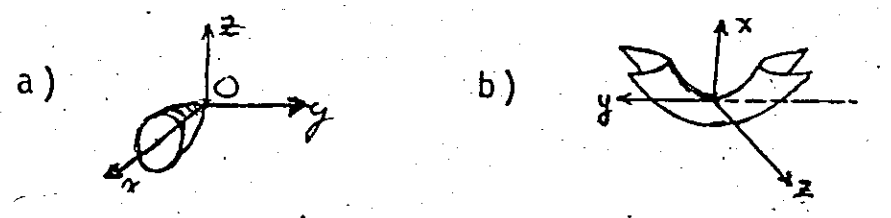
\includegraphics[width=0.6\textwidth]{images/b2p1-262-fig01}

\addtocounter{enumi}{1}
	\item
		By rotation about x-axis by an angle $\pi/4: (x-2)^2+y^{,2}-z^{,2}=4$, hyperboloid of one skeet.

\addtocounter{enumi}{1}
	\item
		$h(x^2+y^2)+2ax(x-h)=0$

\addtocounter{enumi}{1}
	\item
		$(x-a)^2+(y-a)^2=2a^2$

\addtocounter{enumi}{1}
	\item
		$x^2+z^2-y^2=0$ cone

\addtocounter{enumi}{1}
	\item
		$x^2+y^2=(z+1)^2$, cone vertex at $(0,0,-1)$

\addtocounter{enumi}{1}
	\item
		$6y=x^2+9$, parabolic cylinder; \\
		 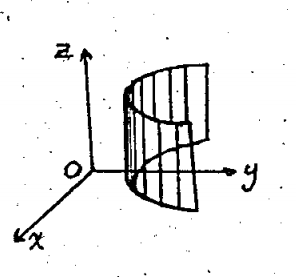
\includegraphics[width=0.2\textwidth]{images/b2p1-262-fig02}

\end{enumerate}

%   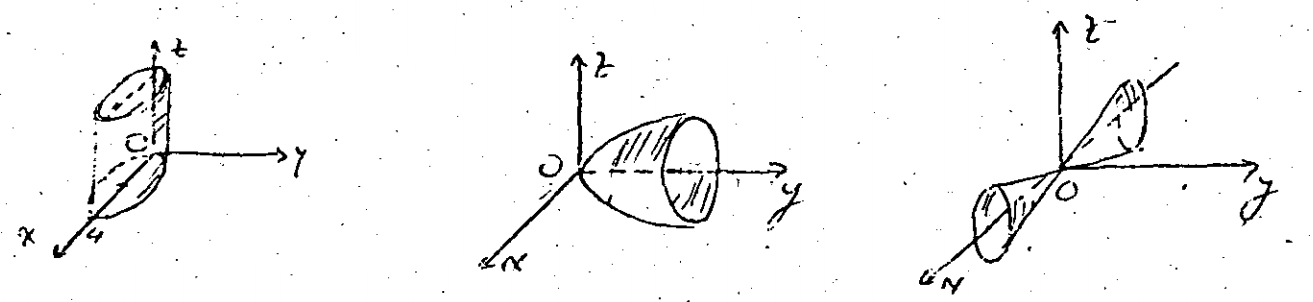
\includegraphics[width=0.9\textwidth]{images/b2p1-221-fig03}
% =======================================================
\end{document}  

